\documentclass{article}
\usepackage{graphicx}
\usepackage{titling}  % For custom title page
\usepackage{circuitikz}
\usepackage{matlab-prettifier}
\usepackage{amsmath}
\usepackage{amssymb}
\usepackage{booktabs,tabu}
\usepackage[section]{placeins}


\title{Experiment 1: Basic Filter Design}
\author{Samyak Sheersh}
\date{2 October 2024}
\newcommand{\subtitle}[1]{%
  \posttitle{%
    \par\end{center}
    \begin{center}\large#1\end{center}
    \vskip0.5em}%
}

\begin{document}

% Custom title page
\begin{titlepage}
    \centering
    
\includegraphics[width=0.2\textwidth]{KGP_logo.png}\par\vspace{1cm}
    {\scshape\LARGE Department of Electronics and Electrical Communication Engineering, IIT Kharagpur\par}
    \vspace{1cm}
    {\huge\bfseries Experiment 4: Speech Recognition with Primarily Temporal Cues\par}
    \vspace{1.5cm}
    {\Large\itshape Samyak Sheersh, Anubhav Mitra\par}
    \vfill
    % Identifying information at the bottom
    {\large Roll Numbers: 22EC30045, 22EC30007\par}
    {\large Group Number: 24\par}
    \vfill
    {\large 2 October 2024\par}
\end{titlepage}

\section{Objectives}
\begin{enumerate}
  \item Generation of multiple frequency bands from the primary signal 
  \item Processing the bands via Hilbert Transform for envelope detection, passing the FFT through an appropriate low pass filter and finally adding noise of the corresponding frequency band to the signal
  \item Qualitative comparison of audio files before and after processing to gauge intelligibility.
\end{enumerate}

\section{Procedure}
\subsection{Generation of bands}
We generate bands on a logarithmic scale. The number of bands is predicted
to have a correlation with the intelligibility of the output, we experiment by
varying this figure from 1 to 16, in a range from 90Hz to 5.76kHz. Notably, a
single band will have one filter of range 90Hz to 5.76Hz, two bands will have
ranges of 90Hz to 720Hz and 720Hz to 5.76kHz.

\subsection{Processing}
We apply a Hilbert Transform to the outputs in their individual bands and
take its magnitude to obtain the envelope of the resultant waveforms in their
respective bands, since the Hilbert transform itself in the time domain can be
conceptualized as the sum of a sine and a cosine component with identical
arguments resulting in a rotating phasor. We then apply a further low-pass
filter of 240Hz, this time on the frequency domain itself to smoothen out any
irregularities present. Finally before recombination, we add white noise whose
band corresponds to the band we are working with.

\subsection{Qualitative Analysis}
The various resultant outputs, sorted by the number of their bands was then
checked for clarity and compared.

\section{Results}
\begin{figure}[!ht]
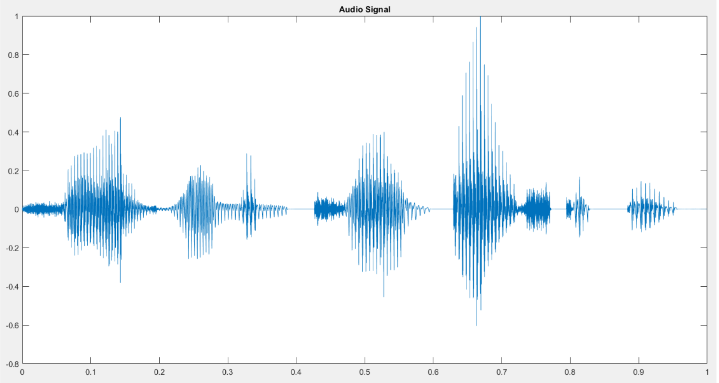
\includegraphics[width=\textwidth]{Signal.png}
\caption{Time plot of the original signal}
\label{fig:sig}
\end{figure}

\begin{figure}[!ht]
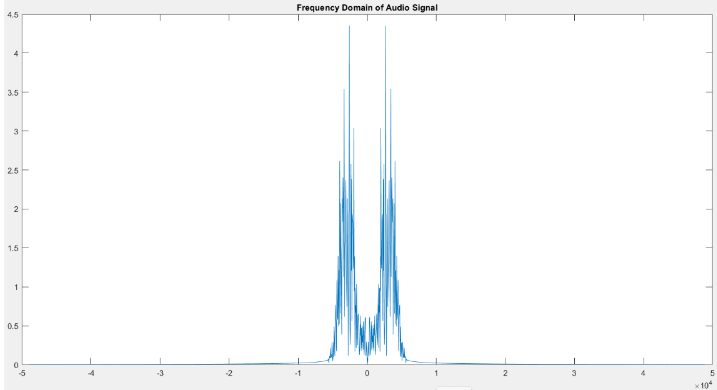
\includegraphics[width=\textwidth]{FFT.png}
\caption{Fourier Transform of the original signal}
\label{fig:FFT}
\end{figure}

\begin{figure}[!ht]
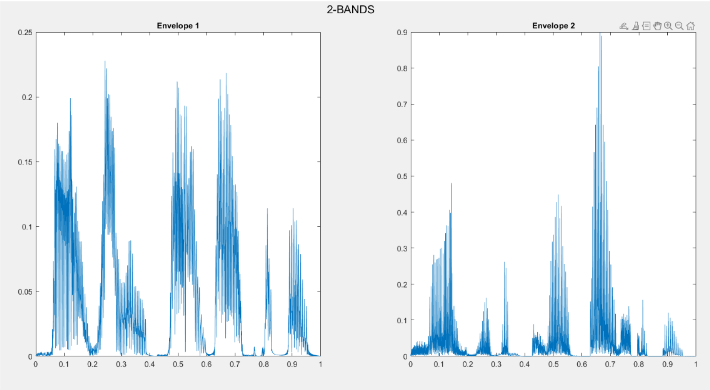
\includegraphics[width=\textwidth]{2_bands.png}
\caption{Time representation of the separated two bands after processing}
\label{fig:2b}
\end{figure}

\begin{figure}[!ht]
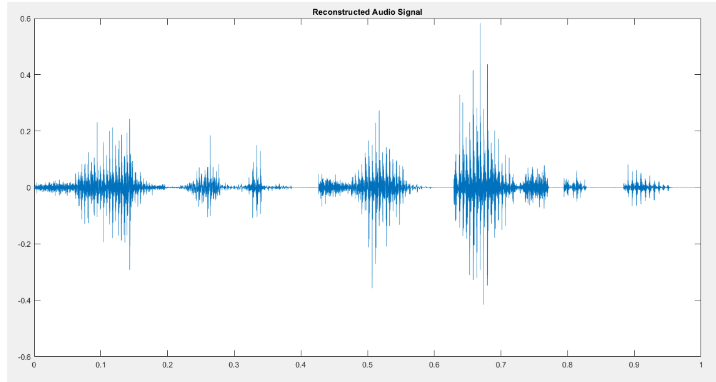
\includegraphics[width=\textwidth]{2br.png}
\caption{Time representation of the reconstructed signal from those two bands}
\label{fig:2br}
\end{figure}

\begin{figure}[!ht]
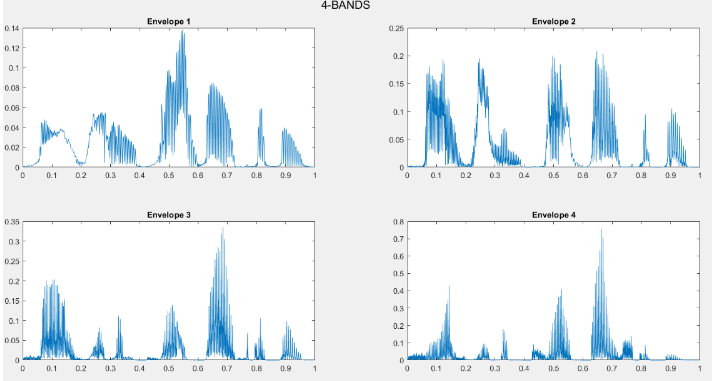
\includegraphics[width=\textwidth]{4_bands.png}
\caption{Time representation of the separated 4 bands post processing}
\label{fig:4b}
\end{figure}

\begin{figure}[!ht]
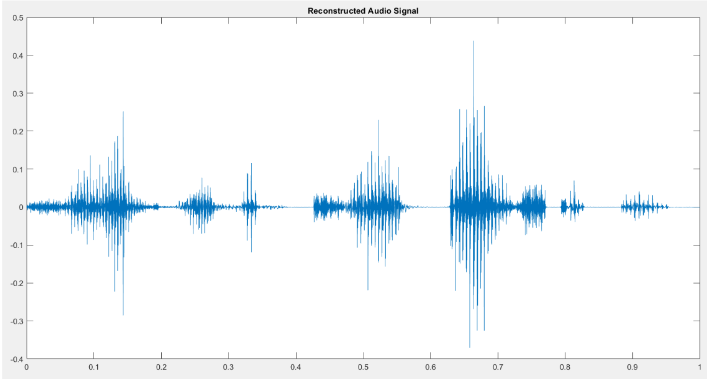
\includegraphics[width=\textwidth]{4br.png}
\caption{Time representation of the reconstructed signal from those 4 bands}
\label{fig:4br}
\end{figure}

\begin{figure}[!ht]
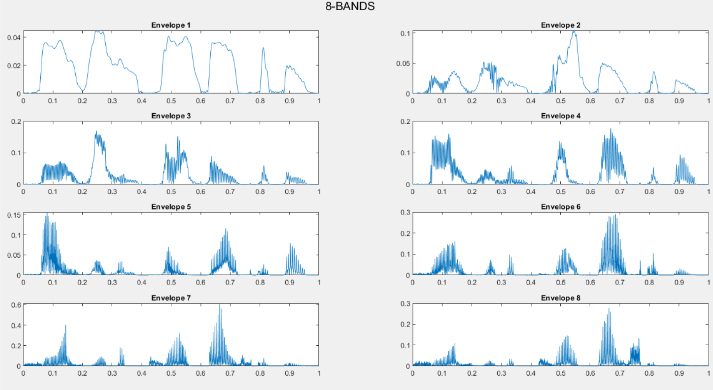
\includegraphics[width=\textwidth]{8_bands.png}
\caption{Time representation of the separated 8 bands post processing}
\label{fig:8b}
\end{figure}

\begin{figure}[!ht]
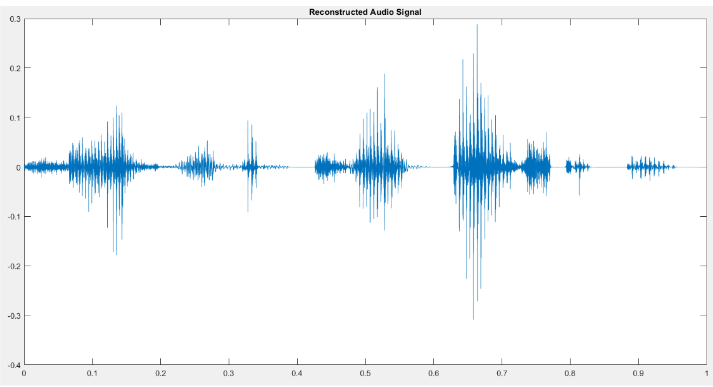
\includegraphics[width=\textwidth]{8br.png}
\caption{Time representation of the reconstructed signal from those 8 bands}
\label{fig:8br}
\end{figure}

\begin{figure}[!ht]
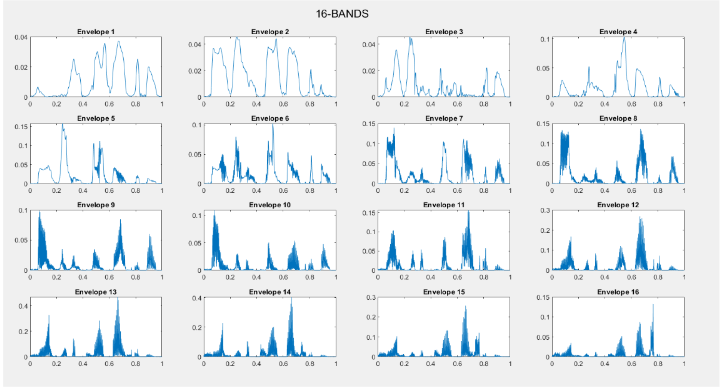
\includegraphics[width=\textwidth]{16_bands.png}
\caption{Time representation of the separated 16 bands post processing}
\label{fig:16b}
\end{figure}

\begin{figure}[!ht]
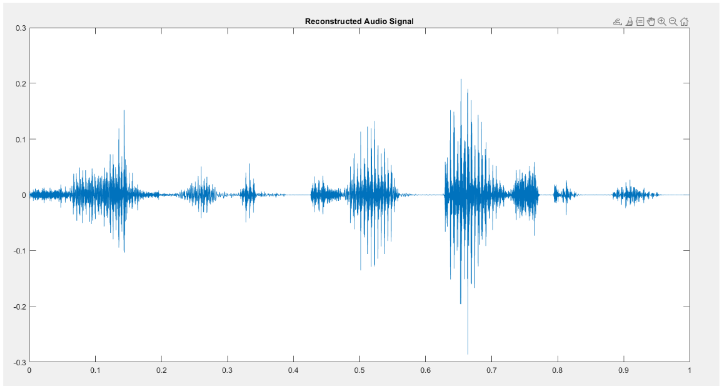
\includegraphics[width=\textwidth]{16br.png}
\caption{Time representation of the reconstructed signal from those 16 bands}
\label{fig:16br}
\end{figure}
\clearpage
\section{Discussion: Samyak Sheersh}
\begin{enumerate}
  \item From the qualitative response (i.e. what we actually heard), we see that as we increase the number of bands, the signal is easier to make sense of. This is because taking a larger number of bands allows us to capture the microstructure of the higher frequencies, and thus we need to reject less actual information and thus the signal is clearer.

  \item However, the fact that we can still make out what is being said points to the fact that the envelope of these sounds is what matters to be intelligible rather than the actual soundwave itself
  \item We used the Hilbert transform to get the envelope for our signal. This is because Hilbert transform (multiplication with $-j.sgn(f)$ in the frequency domain) allows us to obtain what is called an \emph{analytic signal}:
    \begin{equation}
        m_a(t)=m(t) + j m_h(t)
    \end{equation}
    which when we take the modulus, comes out be reasonably accurate since many of the higher order terms become miniscule.
  \item We subsequently multiply this envelope by additive White Gaussian Noise to mimic the natural signal representation of human voice, providing the necessary texture without needing to store the microstructure of the original signal. 
  \item We finally conclude that parallel processing through multiple bands allows us to reproduce human speech in a much more memory efficient manner. 
\end{enumerate}
\end{document}
